\chapter{El reloj de Sol -- I}
\label{sec:el-reloj-de-sol-i}

\lettrine[lines=2]{E}{l día siguiente} encontró a Cecilia y Antonia
ansiosas por atravesar el cuerpo del reloj con todas las horas
diurnas. Cecilia incluso podía sentir en sus manos una delicada
inquietud, casi un fervor, que las sostenía encima del teclado con una
suerte de tensión, como si estuvieran al acecho. Con voz vibrante
anunció a su amiga:

---Creo que ya es tiempo de levantar, con todos los ladrillos que
cocimos hasta aquí, el edificio por el que suspiramos desde
hace\setcounter{m}{\thechapter}\addtocounter{m}{-1} \them{} capítulos.

% ---¡No te olvides del apéndice del Bongo ---recordó Antonia, que
% estaba orgullosa de eso también.

% Cecilia asintió con una enorme sonrisa, mientras arrancaba de las
% teclas alegres chasquidos.


\begin{figure}[ht]
  \begin{minipage}[]{.55\textwidth}%\vspace{0pt}
    \begin{lstlisting}
module reloj_de_sol(){
  difference(){
    cuerpo(170);
    // HACER: Las horas.
  }
}
reloj_de_sol();
    \end{lstlisting}%
  \end{minipage}\hfill
   \begin{minipage}[]{.45\textwidth}%\vspace{0pt}
     \centering
     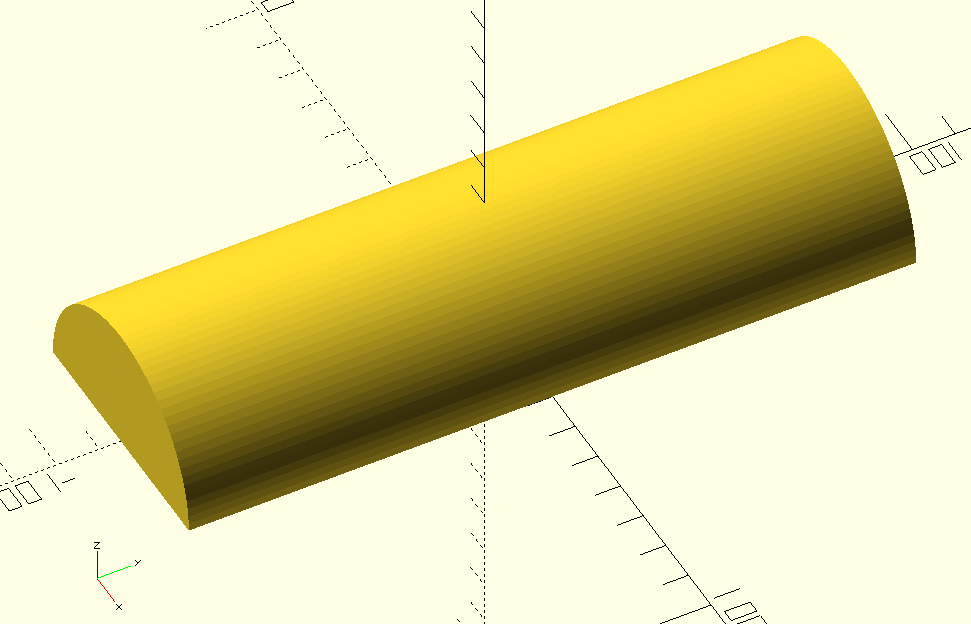
\includegraphics[width=.9\textwidth]{imagenes/cuerpo-del-reloj-a}
\end{minipage}
%\caption{Cecilia y Antonia}
\label{fig:cuerpo-del-reloj-a}
\end{figure}

---¿Por qué `170'? ---objetó Antonia---. Si bien es cierto que en el
capítulo anterior ese valor particular nos sirvió, pensemos que un
eventual lector de nuestro texto quizá quiera modificar los valores de
\lstinline!ancho_pixel! o \lstinline!delta_ancho!, lo cual tornará
obsoleto el caprichosamente específico valor 170.

Cecilia expresó su acuerdo frunciendo los labios; rápidamente esbozó
un dibujo que las ayudara a establecer el largo del cuerpo del reloj
de manera general.

\begin{figure}[ht]
  \centering
  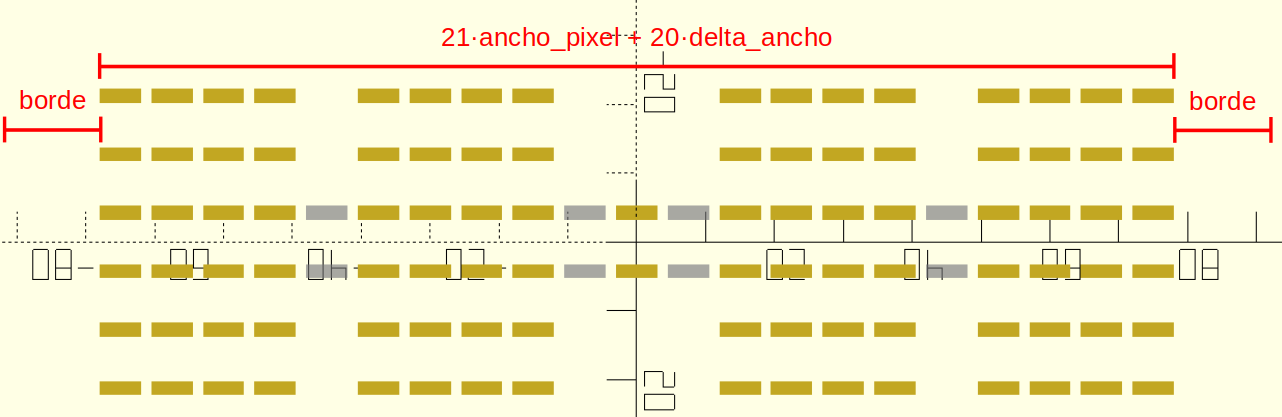
\includegraphics[width=1\textwidth]{imagenes/horas-minutos-largo}
  \caption{Largo del cuerpo del reloj.}
  \label{fig:horas-minutos-largo}
\end{figure} 


---Si no me equivoco, los dígitos con los separadores ocupan
\lstinline!21*ancho_pixel+20*delta_ancho! ---aventuró Cecilia.

Esta vez fue Antonia quien recorrió en silencio y con la punta de sus
dedos el monitor, mientras confirmaba la cuenta de Cecilia:

---Está bueno, además, que permitamos al lector decidir el tamaño del
borde. Quizá quiera escribir en él alguna leyenda: después de todo,
hay una larga tradición de acompañar los relojes de Sol con frases más
o menos profundas... o al menos ingeniosas ---adelantó Antonia.

Cecilia abrió grandes los ojos, dirigiéndolos a su amiga:

---¿Se puede construir texto en \openscad? ---y mientras lo
preguntaba, se dio cuenta de que no podía ser de otra manera: ¿Cómo
podían dejar de lado esa posibilidad los creadores de este hermoso,
potente y dúctil lenguaje..?

---Claro ---confirmó Antonia con una sonrisa---; lo veremos en el
penúltimo capítulo: faltan apenas uno o dos. Bah, en realidad será en
el último: luego vendrá apenas un epílogo, lleno exclusivamente de
pésima literatura y con una sorpresa.

Cecilia recordó la incomodidad que sintiera, en los primeros
capítulos, acerca de las referencias a sus reuniones como secciones de
un manual. Curiosamente, y sin saber muy bien porqué, esas alusiones
ya no la inquietaban tanto.

Antonia, por su parte, ya estaba escribiendo.


\begin{lstlisting}
borde = 0;
largo_reloj = 21*ancho_pixel + 20*delta_ancho + 2*borde;
module reloj_de_sol(){
  difference(){
    cuerpo(largo_reloj);
    hora_solar(12,0);
  }
}
reloj_de_sol();
\end{lstlisting}%

\begin{figure}[ht]
  \centering
  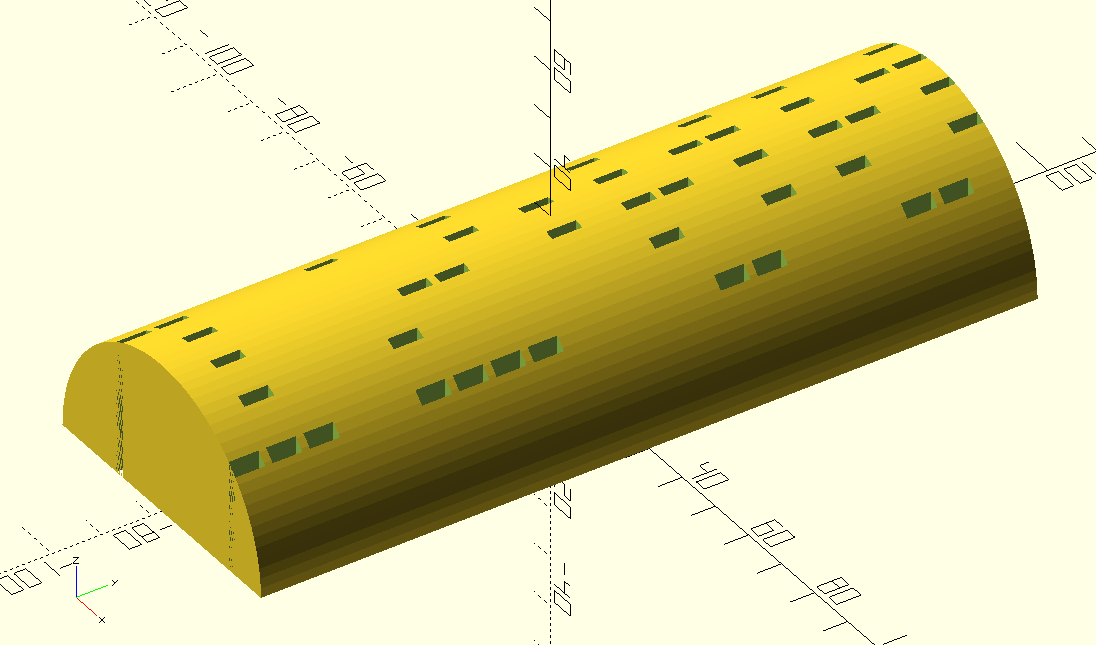
\includegraphics[width=.75\textwidth]{imagenes/cuerpo-del-reloj-b}
  \caption[Largo del reloj II.]{Antonia confirma el largo del cuerpo
    del reloj.}
  \label{fig:cuerpo-del-reloj-b}
\end{figure}
  

---Ahí podemos ver que el `1' está arañando la pared izquierda del
reloj ---señaló Antonia en la figura \ref{fig:cuerpo-del-reloj-b}---;
es lógico, ya que usé un borde nulo a propósito. Lo importante es que
las medidas evidentemente funcionan. Moveré las variables al
principio, junto a las demás, al tiempo que le otorgo a
\lstinline!borde! un valor más sensato ---anunció Antonia.

\begin{lstlisting}
hemisferio="sur";
alto_pixel = 2;
ancho_pixel = 6;
delta_alto  = 6.5;
delta_ancho = 1.5;
borde = 10;
radio_semicilindro = 30;
H = radio_semicilindro+10;
largo_reloj = 21*ancho_pixel + 20*delta_ancho + 2*borde;

//   Mucho texto en el medio

module reloj_de_sol(){
  difference(){
    cuerpo(largo_reloj);
    hora_solar(12,0);
  }
}
reloj_de_sol();
\end{lstlisting}%

\begin{figure}[ht]
  \centering
  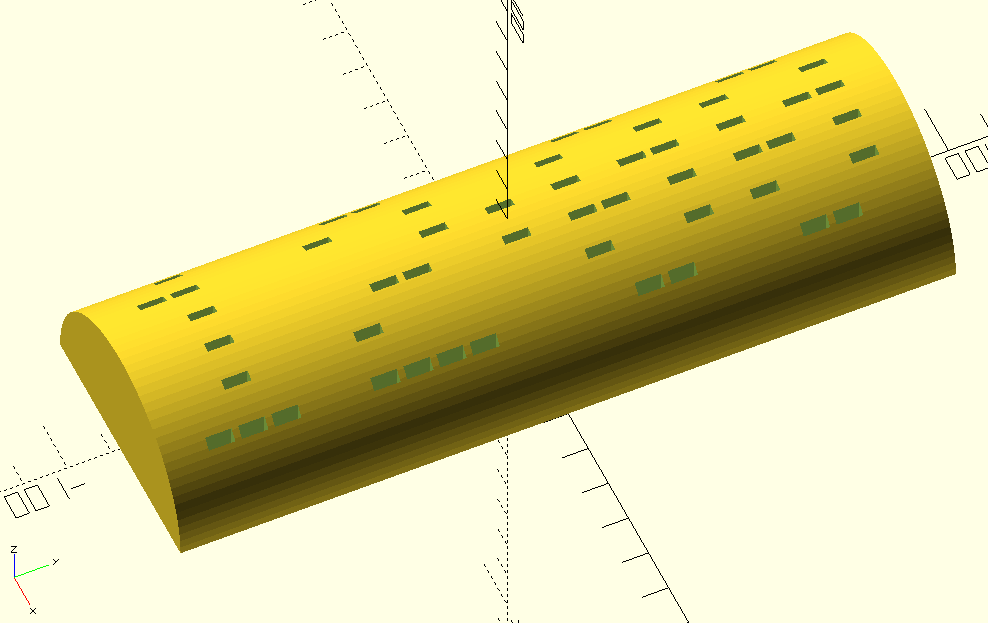
\includegraphics[width=.7\textwidth]{imagenes/cuerpo-del-reloj-c}
  \caption{El largo del reloj abarca ahora sendos bordes.}
  \label{fig:cuerpo-del-reloj-c}
\end{figure}


\section[Un viejo \emph{bug} agazapado]{Un viejo \emph{bug} agazapado
  hace finalmente su aparición}

Cecilia se encontraba exultante; tomó el teclado casi con vehemencia,
decidida a agujerear el reloj con todas las horas desde las 6:00 hasta
las 18:00.


\begin{lstlisting}
module reloj_de_sol(){
  difference(){
    cuerpo(largo_reloj);
    for(horas=[6:17],
        minutos=[0:59])
          hora_solar(horas,minutos);
    hora_solar(18,0);
    }
}
reloj_de_sol();
\end{lstlisting}%

Quizá para crear un clima de tensión dramática, o quizá para
satisfacer la inconsciente y paradójica necesidad que todos, alguna
vez, sentimos por retardar la finalización de un proyecto largamente
acariciado, Cecilia contempló largamente su texto antes de pulsar la
definitiva tecla \keystroke{F5}. Las flamantes líneas 4 y 5 creaban
dos variables, \lstinline!horas! y \lstinline!minutos!, las cuales
recorrían los valores enteros desde el 6 al 17 y desde el 0 hasta el
59, respectivamente. Para cada combinación de ambas variables (en
otras palabras, para todas las horas posibles entre las 6:00 y las
17:59) se restaba al cuerpo del reloj una
\lstinline!hora_solar!. Finalmente se restaba la hora final: las
18:00.

Con la yema del dedo índice ligera y nerviosamente apoyada sobre la
tecla \keystroke{F5}, Cecilia dirigió la mirada a su amiga, en cuyos
ojos creyó percibir el brillo de la misma emoción. En perfecto
silencio, y reclinando levemente la espalda contra el respaldo de la
silla, presionó dicha tecla, dispuesta plenamente a recibir en sus
ojos la felicidad y la dicha bajo la forma de un hermoso reloj de Sol
digital, listo para ser impreso.

Sin embargo, tras unos cuantos minutos fue una desagradable e
inesperada sorpresa la que se desplegó en el monitor frente a su
desconcertada mirada. La figura \ref{fig:reloj-bug-1-2}, por un lado,
mostraba el reloj casi uniformemente barrido por una impiadosa
cuchilla, que eliminó del mismo limpias rebanadas paralelas.


\begin{figure}[ht]
  \centering
  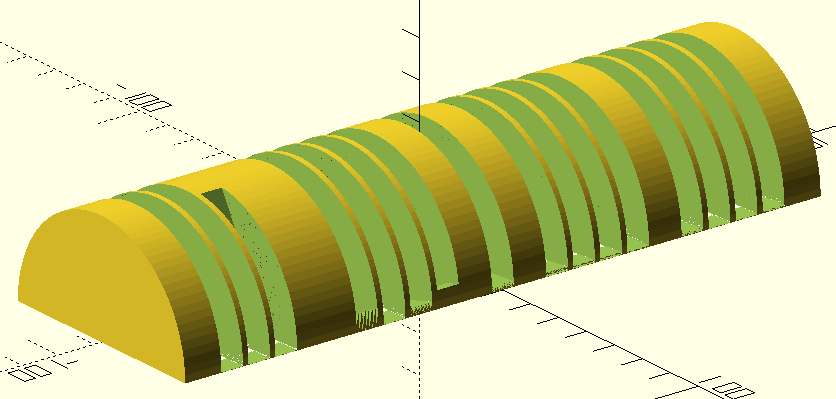
\includegraphics[width=.8\textwidth]{imagenes/reloj-bug-2}
  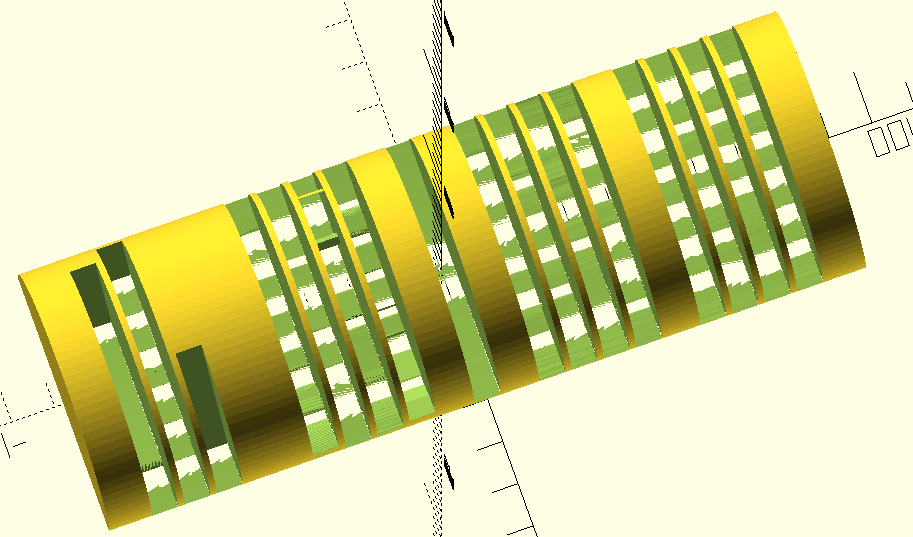
\includegraphics[width=.8\textwidth]{imagenes/reloj-bug-1}
  \caption{Un viejo \emph{bug} hace finalmente su aparición.}
  \label{fig:reloj-bug-1-2}
\end{figure}
  

El otro problema le pareció incluso más urgente y preocupante: en la
consola de mensajes un error campeaba, en un alarmante color rojo y
por duplicado, tal como se puede apreciar en la figura
\ref{fig:reloj-bug-consola}.

\begin{figure}[ht]
  \centering
  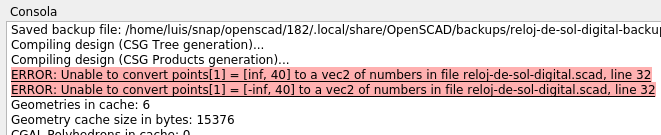
\includegraphics[width=1\textwidth]{imagenes/reloj-bug-consola}
  \caption{Un ominoso mensaje de error aparece en la consola.}
  \label{fig:reloj-bug-consola}
\end{figure}  


En los ojos de Cecilia el brillo confiado del entusiasmo se trocó en
un opaco fulgor de inquieta desazón; giró en dirección a Antonia, en
un instintivo y mudo pedido de auxilio. La encontró sonriendo: era una
sonrisa franca, no burlona; en ella flotaba una delicada expresión de
ternura. Cecilia no tardó en comprender que había caído ingenuamente
en otra trampa, aunque no supo si se la había tendido el reloj o su
amiga.

---Atendamos a un problema a la vez ---empezó An\-to\-nia---; de acuerdo
al mensaje de error de la consola, parece que hubo un problema en la
línea 32 del texto ---y con el mentón señaló el monitor. Cecilia
entendió que eso era una invitación a volver sobre esa línea escrita
tanto tiempo atrás.


\begin{figure}[ht]
  \centering
  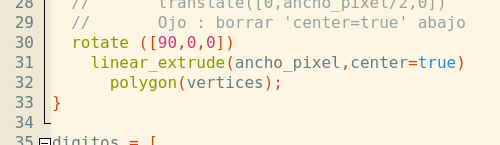
\includegraphics[width=.8\textwidth]{imagenes/bug-linea-32}
  \caption[Línea culpable del \emph{bug}.]{De acuerdo al mensaje de la
    consola en la figura \ref{fig:reloj-bug-consola}, la línea 32 es
    la presunta culpable del \emph{bug}.}
  \label{fig:bug-linea-32}
\end{figure}


Cecilia no podía ver qué problema era capaz de ocurrir en línea tan
inocente como \lstinline!polygon(vertices)!; su gesto de perplejidad
fue tan evidente que hasta Antonia pudo apreciarlo.

---Leamos con atención el mensaje de error de la consola ---pro\-pu\-so
esta última con suavidad---. Parece que hay dos puntos
(\lstinline!points[1] = [inf,40]! y \lstinline!points[1] = [-inf,40]!)
que no pueden ser convertidos a un vector de números...

Antonia adoptaba en su descripción un tono evidentemente didáctico, en
el que Cecilia leía la invitación a descifrar por sí misma el enigma
que tenía delante, a la vez que entendía que el final del reloj se
había alejado una vez más, y que la mejor actitud que debía adoptar
era ni más ni menos que la que las llevó hasta aquí: las ganas de
aprender y superar los obstáculos con confianza y decisión.

Tras volver a leer el mensaje de error, una pregunta se abrió paso con
claridad en su mente:

---¿Qué representan \lstinline!inf! y \lstinline!-inf!? ---inquirió,
sospechando la respuesta.

---Infinito y menos infinito ---respondió lacónicamente Antonia con
una amplia sonrisa, sin duda siguiendo y aprobando el proceso mental
de Cecilia.

---¿Y de dónde pudo haber surgido un infinito..? ---se preguntó ésta
en voz alta. Decidió que quizá sería buena idea indagar de dónde
surgían los \lstinline!vertices! que recibía \lstinline!polygon!.


\begin{figure}[ht]
  \centering
  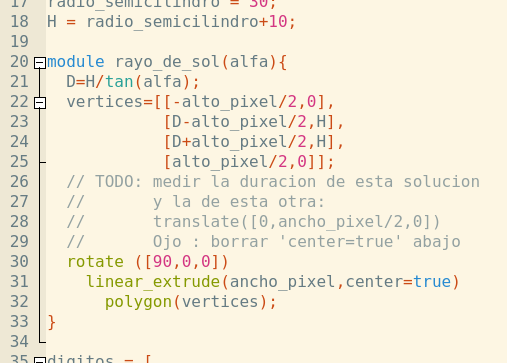
\includegraphics[width=.75\textwidth]{imagenes/bug-linea-32-b}  
  \caption[Origen del \emph{bug}.]{En busca del origen del
    \emph{bug}.}
  \label{fig:bug-linea-32-b}
\end{figure}


Los \lstinline!vertices! procedían ---como podía apreciarse en el
texto en la figura \ref{fig:bug-linea-32-b}--- de las líneas 22 a 25;
nada anómalo parecía haber en ellas: \lstinline!alto_pixel! y
\lstinline!H!  eran parámetros iniciales que no podían dar lugar a
ninguna clase de infinito, y \lstinline!D! era calculado en la línea
21... En ese momento, los ojos de Cecilia se abrieron como dos soles
que quisieran abrasar el monitor: ¡En el cálculo de \lstinline!D! se
empleaba la función \lstinline!tangente!! Si \lstinline!tan(alfa)!
fuera nulo...

---Antonia, ¿es posible que en \openscad{} la división por cero arroje
como resultado infinito? ---conjeturó instintivamente Cecilia,
respondiendo a una vehemente corazonada.

La sonrisa de Antonia no podía ser más amplia:

---Sí, es exactamente así; mirá: ---y tomando el teclado lo confirmó
con un par de ejemplos.\footnote{¡Ah, no! !$\frac{1}{0}=\infty$! ¡Esto
  es demasiado!  ¡Renuncio! (Nota del Editor)}$^,$\footnote{No,
  editor... daaleee... quedate. (Nota de Cecilia, Antonia y
  Luis)}$^,$\footnote{Uh... ¿En serio quieren que me quede? (Nota del
  Editor)}$^,$\footnote{¡Pero claro que sí! (Nota de Antonia, Cecilia
  y Luis)}$^,$\footnote{Bueno: me quedo \Changey{2}. (Nota del
  Editor)}

\begin{center}
  \begin{minipage}[]{.45\textwidth}%\vspace{0pt}
    \begin{lstlisting}
echo(1/0,-8/0);
    \end{lstlisting}%
  \end{minipage}\hfill
  %\begin{center}
   \begin{minipage}[]{.55\textwidth}%\vspace{0pt}
       \centering
       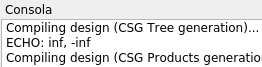
\includegraphics[width=1\textwidth]{imagenes/infinitos}
\end{minipage}
\end{center}

Cecilia recobró gran parte de su confianza al haber dado al menos con
el origen del error; ahora tenía por delante, eso sí, la tarea de
solucionarlo. Recordó que \lstinline!tan(alfa)! sólo podía valer 0 si
\lstinline!alfa==0! o \lstinline!alfa==180!: ¿En qué condiciones los
rayos de Sol caían con esos ángulos? Buscó la respuesta en el capítulo
\ref{cap:poquito-de-astronomia}; la encontró en la figura que copiamos
como \ref{fig:sol-15-horas-bug}.


\begin{figure}[ht]
  \centering
  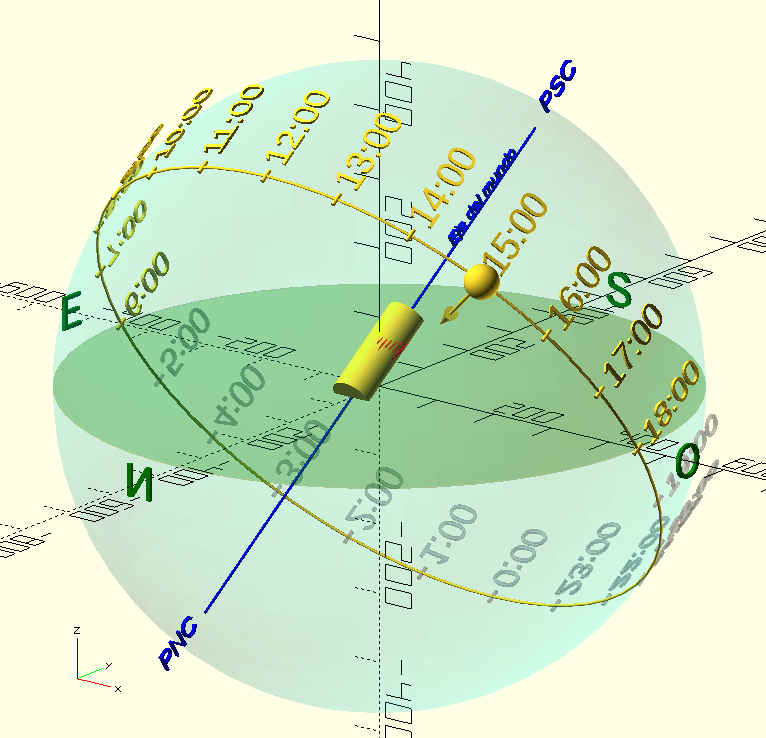
\includegraphics[width=.6\textwidth]{imagenes/sol-15-horas.png}  
  \caption{A las 6:00 y a las 18:00 los rayos del Sol forman un ángulo
    nulo respecto del plano \coord{XY}.}
  \label{fig:sol-15-horas-bug}
\end{figure}


---¡Claro! ---Cecilia ya estaba nuevamente en vena---.  Un ángulo de
0$^{\circ}$ o 180$^{\circ}$ corresponden a rayos rasantes respecto de
la base del reloj... ¡O sea que ocurren a las 6:00 y a las 18:00!

Con una amplia sonrisa de satisfacción, e irguiendo los hombros con
renovada seguridad, Cecilia propuso:

---¡Listo, Antonia! Con evitar las 6:00 y las 18:00 solucionamos ese
problema.

---Sí... ---Antonia asintió con desgano---. Podemos hacer eso y
desentendernos del mismo; pero el problema, considerado en sí mismo,
seguirá ahí, en el texto.

---¿Pretendés acaso modificar el comportamiento de la función
\lstinline!tangente!? ---preguntó Cecilia, extrañada y un poco
mortificada por no haber recibido la felicitación que esperaba de su
amiga.

---¡Claro que no! ---protestó Antonia---. No me refiero a eso. Quiero
decir que debemos anticipar que el eventual lector de nuestro texto no
caiga en el mismo error y la misma perplejidad que nos detuvo por unos
momentos. Y recordá que nosotras mismas seremos también nuevas
lectoras, cuando nos enfrentemos a nuestra propia obra en un par de
meses.

---Nadie se baña dos veces en el mismo río, ¿no? ---comentó Cecilia,
que sabía que esta frase de Heráclito era una de las preferidas de
Antonia: al menos, una de las tantas que la acompañaban y le gustaba
recordar.

Antonia sonrió dulcemente, mientras asentía:

---Porque el río no es el mismo, ni una es la misma...

\section{\texttt{assert}}

---En general, los mensajes de error de \openscad{}, como ya pudiste
comprobar, no sólo son bastante crípticos sino que rara vez apuntan al
origen de los problemas: más bien señalan la línea donde finalmente se
manifiestan y explotan ---Antonia inició otra de sus explicaciones
retomando el tono didáctico---. Ahora bien, cuando una sabe que cierta
función o módulo debe recibir parámetros que respondan a determinadas
condiciones, y que en caso de que no se cumplan el proceso de
construcción no debe continuar, resulta utilísima la sentencia
\lstinline!assert! ---y tecleó con rapidez otro de sus ejemplos
vanales.

%\begin{center}
  \begin{minipage}[]{.62\textwidth}%\vspace{0pt}
    \begin{lstlisting}
module prueba(a){
  assert(a!=0,"el parametro 'a' no debe ser cero");
  cube(20);
} 
prueba(a=0);
    \end{lstlisting}%
  \end{minipage}\hfill
  %\begin{center}
   \begin{minipage}[]{.37\textwidth}%\vspace{0pt}
       \centering
       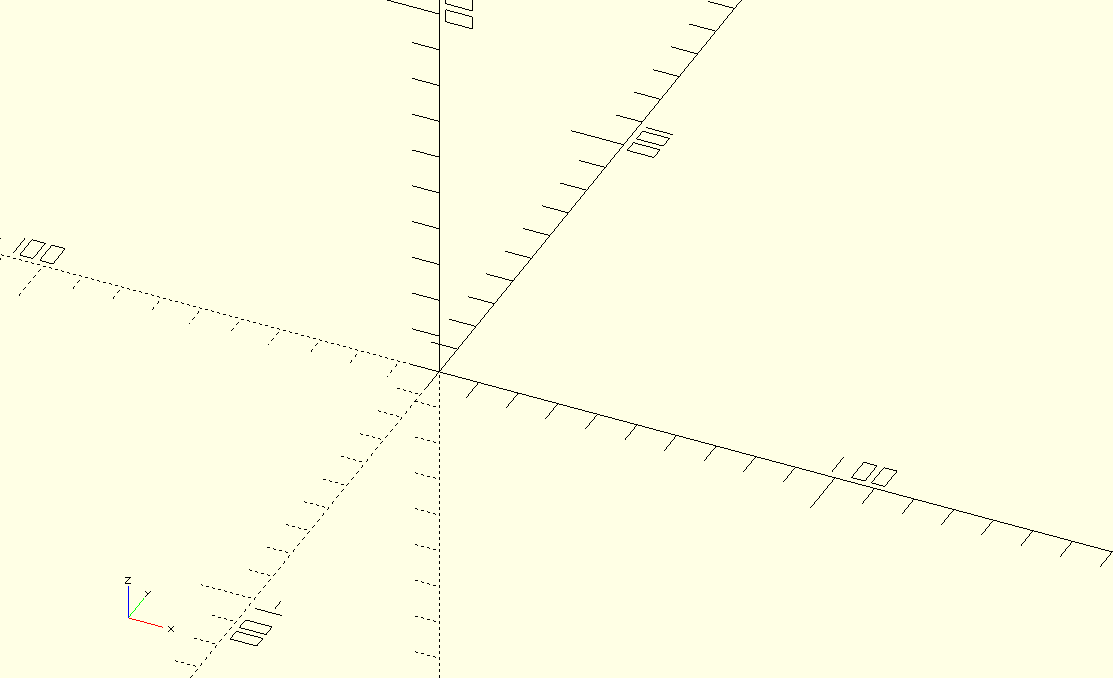
\includegraphics[width=.85\textwidth]{imagenes/vacio}
\end{minipage}
%\end{center}

\begin{figure}[ht]
  \centering
  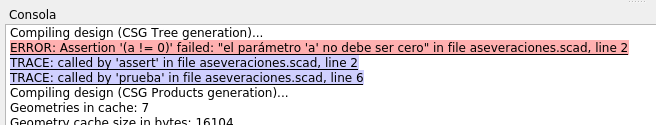
\includegraphics[width=1\textwidth]{imagenes/assert-1}  
  \caption{\texttt{Assert}.}
  \label{fig:assert-1}
\end{figure}


Antonia permitió que Cecilia contemplara el texto y el mensaje de la
consola en la figura \ref{fig:assert-1} unos momentos antes de
continuar:

---La idea es ésta: \lstinline!assert!  admite dos parámetros: el
primero es una condición a evaluar (en nuesto caso, \texttt{a!=0}). Si
la misma es verdadera, todo bien: \openscad{} prosigue con el resto de
las instrucciones. Pero si es falsa, detiene la construcción con un
mensaje de error, cuyo texto se corresponde con el segundo parámetro
que vos le pasaste a \lstinline!assert!. De esa manera, no sólo
impedís que se lleve a cabo una construcción probablemente anómala
sino que recibís un mensaje de error un poco más expresivo y certero.

A Cecilia le pareció bastante útil:

---Entonces se trata de anticipar los valores extremos
\lstinline!alfa==0! y \lstinline!alfa==180! ---dijo, y recobrando el
teclado propuso la siguiente modificación:

\begin{lstlisting}
module rayo_de_sol(alfa){
  assert(alfa!=0 && alfa!=180, "'alfa' no debe ser nulo ni llano.");
  D=H/tan(alfa);
  vertices=[[-alto_pixel/2,0],
            [D-alto_pixel/2,H],
            [D+alto_pixel/2,H],
            [alto_pixel/2,0]];
  // TODO: medir la duracion de esta solucion
  //       y la de esta otra:
  //       translate([0,ancho_pixel/2,0])
  //       Ojo : borrar 'center=true' abajo
  rotate ([90,0,0])
    linear_extrude(ancho_pixel,center=true)
      polygon(vertices);
}
// Varias lineas de texto
module reloj_de_sol(){
  difference(){
    cuerpo(largo_reloj);
    hora_solar(6,0);
  }
}
reloj_de_sol();
\end{lstlisting}%


\begin{figure}[ht]
  \centering
  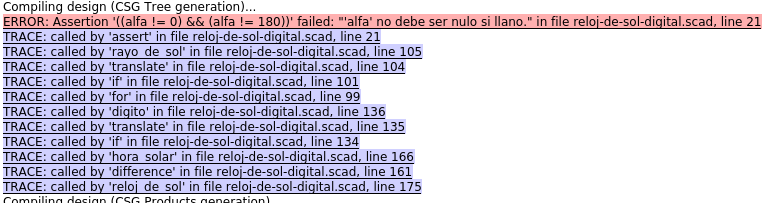
\includegraphics[width=1\textwidth]{imagenes/assert-2}  
  \caption{\texttt{Assert} impide que el usuario trate de horadar el reloj con
    rayos paralelos al horizonte.}
\label{fig:assert-2}
\end{figure}


A Cecilia, mientras contemplaba la figura \ref{fig:assert-2}, le gustó
el hecho de que \lstinline!assert! revelara también toda la cadena de
llamadas entre funciones y módulos que condujeron al espantable error:
en más de una oportunidad podría tratarse de información muy
relevante.

Antonia miraba el monitor con un gesto indeciso:

---La condición está bien ---admitió---; el rayo de Sol sólo puede
crearse si \texttt{alfa!=0} y \texttt{alfa!=180}.  Sin embargo,
imagino que el lector de este texto no necesariamente esté interesado
en el ángulo alfa: quizá piense más en términos de `horas' y
`minutos', que son los que finalmente querrá ver expresados en el
reloj. Lo que quiero decir es que cualquier información sobre el
ángulo seguramente le resultará tan inexpresiva como la alusión
original a los infinitos que, por defecto, lanzó \openscad.

Cecilia comprendió el punto: el ángulo alfa no era más que un detalle
de la implementación interna del algoritmo. Tras recorrer nuevamente
el texto, decidió que el responsable de comprobar la validez de la
hora era el módulo \lstinline!hora_solar!, por lo que luego de
deshacer la modificación introducida en \lstinline!rayo_de_sol!
compartió el siguiente texto con Antonia:

\begin{lstlisting}
module hora_solar(horas,minutos){
  hora=horas+minutos/60;
  assert(hora!=6 && hora!=18,"La hora no debe ser las 6:00 ni las 18:00.");
  alfa=alfa(hora);
  hora_decenas=n_a_digito(horas,1);
  hora_unidades=n_a_digito(horas,0);
  minuto_decenas=n_a_digito(minutos,1);
  minuto_unidades=n_a_digito(minutos,0);
  // Varias lineas de texto
}
module reloj_de_sol(){
  difference(){
    cuerpo(largo_reloj);
    hora_solar(18,0);
  }
}
reloj_de_sol();
\end{lstlisting}%


\begin{figure}[ht]
  \centering 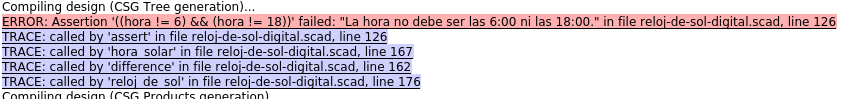
\includegraphics[width=1\textwidth]{imagenes/assert-3}
  \caption{Cecilia desplaza el \texttt{assert} al módulo
    \lstinline!hora_solar!.}
  \label{fig:assert-3}
\end{figure}



Como el valor de la \lstinline!hora! debía usarse tantas veces,
Cecilia decidió además realizar su cálculo al principio, en la línea
2. No sin recelo dirigió la mirada en dirección a su amiga: encontró
en ella nuevamente una expresión no del todo satisfecha.

---¿Sabés qué? ---adelantó Antonia---. Ya que estamos, podríamos
impedir también la mera posibilidad de que algún lector descuidado
pretenda agujerear el reloj `desde abajo', pasando horas previas a las
6:00 o posteriores a las 18:00... ¿No te parece?

Cecilia suspiró con ostensible cansancio; mas debía reconocer que, muy
a su pesar, la propuesta de Antonia era bastante razonable. En
cualquier caso, implementar esa precaución no le pareció muy difícil,
y confió en que ya le quedaran pocas páginas al capítulo.

\begin{lstlisting}
module hora_solar(horas,minutos){
  hora=horas+minutos/60;
  assert(hora>6 && hora<18,"La hora debe encontrarse entre las 6:00 y las 18:00.");
  alfa=alfa(hora);
  hora_decenas=n_a_digito(horas,1);
  hora_unidades=n_a_digito(horas,0);
  minuto_decenas=n_a_digito(minutos,1);
  minuto_unidades=n_a_digito(minutos,0);
// Varias lineas de texto
module reloj_de_sol(){
  difference(){
    cuerpo(largo_reloj);
    hora_solar(21,0);
  }
}
reloj_de_sol();
\end{lstlisting}%


\begin{figure}[ht]
  \centering
  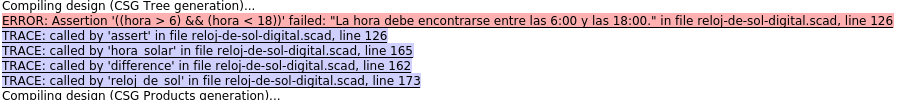
\includegraphics[width=1\textwidth]{imagenes/assert-4}  
  \caption{De puro precavidas, Antonia y Cecilia deciden evitar
    incluso la posibilidad de que un usuario pretenda agujerear horas
    nocturnas.}
  \label{fig:assert-4}
\end{figure}


Antonia, ahora sí, demostró su conformidad asintiendo con una
sonrisa.

---Ya sabemos cómo impedir las horas conflictivas ---a\-pro\-bó---; ahora deberíamos asegurarnos de que el resto es
aceptado por el módulo \lstinline!reloj_de_sol!.

Cecilia estuvo a punto de decir que sí, pero algo la inquietaba desde
hacía rato, sin que pudiera definir muy bien qué. Tenía que ver con el
error que acababan, presumiblemente al menos, de resolver; tenía que
ver con la \lstinline!tangente!...

---¡Pará! ---lanzó Cecilia, tomando conciencia de pronto del problema
que bullía en su inconsciente---. La función \lstinline!tangente! no
sólo puede devolver un confictivo 0, sino un aún más problemático
`infinito'... ¡Y de hecho lo hace para 90$^{\circ}$! ¡Nada menos que a
pleno mediodía! ---Cecilia sintió un escalofrío que la obnubiló e
impidió recordar que varias veces habían probado ya esa hora
meridiana; se lanzó así sobre el teclado casi con la seguridad de ver
aparecer otro error:

\begin{lstlisting}
module reloj_de_sol(){
  difference(){
    cuerpo(largo_reloj);
    hora_solar(12,0);
  }
}
reloj_de_sol();
\end{lstlisting}%

\begin{figure}[ht]
  \centering
  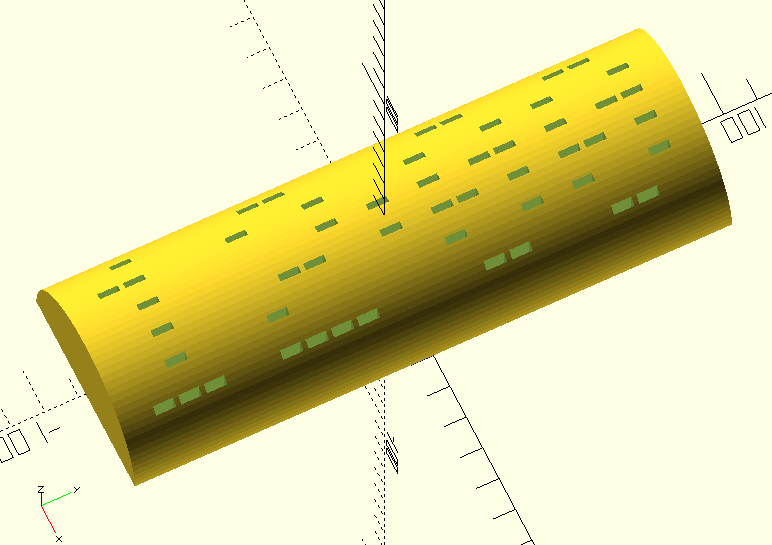
\includegraphics[width=.75\textwidth]{imagenes/12_00-a}  
  \caption{Las 12:00 son representadas apaciblemente por el módulo
    \lstinline!reloj_de_sol! aun cuando la tangente de $90^{\circ}$ no
    tenga solución en los números reales.}
  \label{fig:12_00-a}
\end{figure}

La tranquila aparición de las 12:00 en la figura \ref{fig:12_00-a}
sólo contribuyó a confundirla más. Antonia tomó suavemente el teclado,
mientras explicaba:

---Efectivamente, \openscad{} sabe perfectamente que
\lstinline!tan(90)! no tiene solución en los números reales, y lo
expresa a su modo:


\begin{figure}[ht]
  \begin{minipage}[]{.4\textwidth}
\begin{lstlisting}[numbers=none]
echo(tan(90));
\end{lstlisting}%
  \end{minipage}\hfill
  \begin{minipage}[]{.6\textwidth}
    \centering
  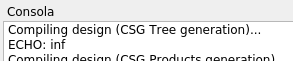
\includegraphics[width=.9\textwidth]{imagenes/tangente-90}  
  \end{minipage}
  \caption{\openscad{} adopta la convención de que
    $\tan 90^{\circ}=\infty$.}
  \label{fig:tangente-90}
\end{figure}


\guillemotright La cuestión es que si dividís un número real por
`infinito' en \openscad{}, obtenés 0 ---aclaró Antonia\footnote{¡Que
  conste que me quedo sólo porque me lo pidieron! (Nota del
  Editor)}---.  Es... raro, lo admito; pero no podemos negar que
resulta conveniente y hasta intuitivo, sobre todo en un dominio
claramente más geométrico que aritmético ---añadió, alzándose de
hombros y buscando la complicidad de Cecilia, quien con un suspiro de
alivio y alzando los ojos al techo expresó con claridad que estaba de
acuerdo, quizá más por cansancio que por convicción algebraica.




\begin{figure}[ht]
  \begin{minipage}[]{.4\textwidth}
\begin{lstlisting}[numbers=none]
echo(1/tan(90));
\end{lstlisting}%
  \end{minipage}\hfill
  \begin{minipage}[]{.6\textwidth}
    \centering
  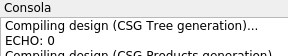
\includegraphics[width=.9\textwidth]{imagenes/tangente-90-a}  
  \end{minipage}
  \caption{Para escándalo de los matemáticos, en \openscad{}
    $\frac{1}{\tan 90^{\circ}}=0$.}%\iftoggle{libro}{}{\vspace{128in}}
  \label{fig:tangente-90-a}
\end{figure}

---¿Te parece que dejemos la solución del otro problema para el
capítulo que viene? ---propuso Antonia, y a Cecilia nuevamente no le
costó nada estar de acuerdo de todo corazón.






%%% Local Variables:
%%% mode: latex
%%% TeX-master: "../libro"
%%% End:
